\documentclass[12pt, twoside]{article}
\usepackage{geometry}
\usepackage{caption}
\usepackage{subcaption}
\geometry{a4paper}

\usepackage[mono=false]{libertine} 

\usepackage{amsfonts}
\usepackage{amsmath}
\usepackage{amssymb}
\usepackage{amsthm}
\usepackage{etoc}

\usepackage[toc,title,titletoc,header]{appendix}
\usepackage{minitoc}
\usepackage{cancel}
\usepackage{imakeidx} % before hyperref
\usepackage{hyperref}
\usepackage{graphicx}
\usepackage{wrapfig}
\graphicspath{ {img/} }
\usepackage{verbatim}
\usepackage{setspace}
\usepackage{epigraph}
\usepackage[english]{babel}
\usepackage[T1]{fontenc}
\usepackage[utf8]{inputenc}
\usepackage{a4}
\usepackage{csquotes}
\usepackage{url}
\usepackage{lettrine}
\usepackage{graphicx}
\usepackage{lscape}
\usepackage{epsfig}
\usepackage{epstopdf}
\usepackage{eurosym}
\usepackage{booktabs}
\usepackage{enumitem}
\usepackage{multirow}
\usepackage{multicol}
\usepackage{lscape}

\newenvironment{footcitedquote}[1][]
  {% \begin{footcitedquote}[.]
   \let\mkcitation\footnote% Citations will be footnotes
   \def\optarg{#1}% Capture optional argument
   % Set up start of displayquote environment
   \edef\envstart{\noexpand\begin{displayquote}\if$\optarg$\else[\noexpand\optarg]\fi}%
   \envstart}
  {\end{displayquote}}% \end{footcitedquote}

\title{Zillow’s Home Value Prediction}
\author{Matteo Spanio}
\date{Settembre 2022}


\begin{document}
  \begin{titlepage}
    \begin{center}
        
\includegraphics[width=0.6\textwidth]{img/long_logo.jpg}
        
        \vspace{2.5cm}
        \Huge
        \textbf{Data and Web mining}
 
        \vspace{0.5cm}
        \LARGE
 
        \vspace{1cm}
 
        \textbf{Prof. Claudio Lucchese}
 
        \vfill
 
        Zillow’s Home Value Prediction
        
        \vfill

        \textbf{Matteo Spanio}\\
        {Matricola: 877485}
 

        \vspace{0.8cm}
        \Large
        Settembre 2022
 
    \end{center}
\end{titlepage}

  \onehalfspacing

  \section{The dataset}
     
  The first problem to consider was how to join the data, the dataset is a collection of houses features splitted by year of assessment. Should I make an analysis for each year or merge the datasets togheter? How to handle duplicated rows?
    
There could be different trends in different years and create a single model could be a bad idea, anyway at a first sight the dataset is quite homogeneous, so I decided to merge all togheter. In second instance I saw that there were some duplicated rows, actually few hundreds of houses have been sold twice or trice in a year: keep them all could create redundancy and alter the columns statistics, nevertheless we could find some interesting information about the variations (or non-variations) of error over time, so I decided to keep them all\footnote{
    Also the Zillow competition expects to predict the sell value of a property in different months and years, so I assume it is important to keep the information about the time of the assessment.
    }.

\subsection{Features}

After studying about the functioning of the division by American geographical and administrative areas and the structure of the most common houses in America, I figured out that some columns were in reality duplicated data: a lot of administrative subdivision were redundant and probably not necessary, since we already have a fine grained location data given by coordinates probably a city id or the neighborhood id were not necessary, so I dropped those columns and other administrative categories. Also some other features were duplicated since Zillow provided the raw data they get from assessors and ones calculated by themselves\footnote{see in the comment section at \url{https://www.kaggle.com/c/zillow-prize-1/discussion/33899} for more informations.}.

Hence we can see that many rows are missing some values. Diving deep in the problem we can infer that many columns probably\footnote{Here I used the word ``probably'' because we don't really know if missing values were zero or there were some other kind of issue so that the real value was not taken, anyway, based on statistics and logic, it is likely that more houses paid the taxes or didn't have a spa} did not input data when the value was zero (it is not a all comprehensive case, some features were relevant only for certain counties, see more at \ref{counties_importance}). For example, if a house does not have a spa, the value of the column ``spa'' is missing, but it is not zero. For categorical data I decided to fill the missing values with zero, since it is the most likely value, while fill continuous data was more thought. Some columns are missing a lot of fields where others are just missing few hundreds or thousands of rows. I decided to fill the least unpopulated columns with their mean\footnote{Actually not the exact mean, I used instead the following formula:
$$
    x_{\text{NaN}} = \left\lfloor \frac{1}{n} \sum_{i=1}^{n} x_i \right\rfloor
$$
where $n = |\text{column}|$ and $x_i \neq \text{NaN}$. Since I replaced every column with the same function I included the floor function because some features are integers (e. g. year) and other data are not really messed up if I drop some decimals after floating point (e. g. $853$ square feets is almost the same information as $853.37$ square feets, and the same is for values in dollars).}, and for each touched feature I added a column to mark if the data has been altered --- to be able to recognise if a specific feature was missing could be significant since we are trying to predict the prediction error of \textit{Zestimate} (see more about crafted features at \ref{crafted_features}).

\subsection{Are counties relevant?}\label{counties_importance}

Plotting the data divided by county it came out that some of the most unpopulated features where taken only for certain counties, and here comes a new problem: how to handle those missing values? I didn't like too much remove columns that can be useful, especially if they were complete for some categories of data. The solution I embraced was to split data into specialized analysis: I filtered the data by county and created a model for each county.
This solution has some drawbacks: the models are not comparable and the dataset is not homogeneous, anyway we can take advantage of more features and we can see also that some trends are going on, the county of Los Angeles has more records, but also the greatest variance of data (more about data inference at \ref{conclusions}).
    
To be fair a good model should be able to detect differences between counties if there are any, but I didn't came to a solution that could take into account different features in the same model. I ended up creating four models, one for each county and one for the whole dataset.

\subsection{Response variable}

Once I was done filling gaps in the dataset and ready to start making predictions I asked myself: is the $\log{error}$ a good quantity to make predictions on? What could happen if I transform the response variable?

By definition the $\log{error}$ is the difference between the predicted value and the real value, for the properties of logarithm it means that is the logarithm of the relationship between the two values:
$$
\begin{aligned}
    &\log error = \log(Zestimate) - \log(SalePrice)\\
    = \log{\left(\frac{Zestimate}{SalePrice}\right)} &\sim
    \mathcal{N}\left(\frac{\sum_{i=1}^n x_i}{n}, \frac{\sum_{i=1}^n x_i^2 - \bar {x}} {n-1}\right)\quad\text{where }x = \log error 
\end{aligned}
$$
in this case we take into account the logarithm of a ratio because it better approximates to a normal distribution and it is homoscedastic. We could have taken in consideration different data transformations, but most of the time it would have been an unequous choice: the logarithm stretches the interval $[0, 1]$ to $]-\infty, 0]$ and reduces the distance between data $> 1$, while a square root would have also reduced data $>1$ but data in $[0,1]$ would have been more close to each other, with the possibility to make predictions of understimations harder.



  \section{Model selection}

  \subsection{Model measure}

    
Per le predizioni sono stati presi in considerazione più modelli di regressione, la predizione di base su cui misurare le altre è 

There is evidence that there are many differences between counties, but the models didn't catch it.

  \section{Conclusions}\label{conclusions}
    
  As we can see from ensemble models tuning and performance we weren't able to decrease variance or bias of our predictions. So the question is: is there any possibility to reduce the prediction error?
We know from theory that:

$$\text{Error}(\mathcal{M} ) = \text{Bias}^2 + \text{Variance} + \varepsilon$$
since we know that boosting should reduce the bias and bagging (random forests) should reduce the variance, we can conclude that the error is not going to decrease, in fact we have not been able to reduce the error beyond a certain threshold that is probably the value of $\varepsilon$ in the previous formula.

  \begin{figure}[h]
    \centering
    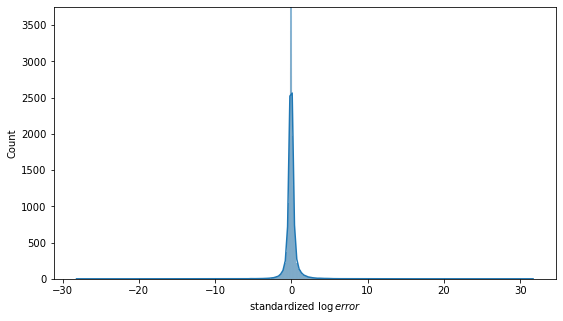
\includegraphics[width=0.8\textwidth]{img/standard_log_error_dist.png}
    \caption{Standardized distribution of the log error}
  \end{figure}

The distribution of data confirms this thesis: standardizing the distribution of the $\log error$ we get a normal distribution with mean 0 and variance 1, but with extremely long tails (data goes from $-30$ to $30$). The fact is that predict an error $e$ such that $|e| > 4$ in a standard normal distribution is nearly impossible, we have to conclude that those tails include many outliers (or data from another kind of distribution) and that the model is not able to predict them.

The problem is that houses with wrong error prediction are not really different from other ones. If we assume that most of the errors have been made by humans\footnote{Often in large dataset problems come from data input. In this case we have a confirm from this conversation (\url{https://www.kaggle.com/competitions/zillow-prize-1/discussion/36752}), where we read that it's more likely that when Zestimate gets a high error in reality it did well, while the sell price in the database was inserted with an error.} it is not a surprise to see that errors are most incident where there are more data (imagine who inputs a lot of data has an high chance to input something wrong) and we still get that the error due to data input is not predictable.

The conclusions of this analysis have led us to this point, this does not mean that the work to predict the log error is finished, here is a list of possible steps from which to start for further investigations:

\begin{itemize}
  \item perhaps data cleaning was not adeguate, try removing data in a different way;
  \item we found that predict outliers is nearly impossible, we could drop them or create a specialized model for outliers;
  \item try focus on new features based on the features importance we got from the analysis, it could be that a ratio $taxes assessed \over sqare feets$ have an impact on prediction;
  \item apply different transformations on data to change their distribution.
\end{itemize}


\end{document}